\documentclass[../main.tex]{subfiles}

\begin{document}

\chapter{Pilot Experiments Design and Results}

This chapter describes the experimental design for the evaluation of the
fluctuation strength attribute. First, the initial design (as
in~\cite{Fastl1982Fluctuation}) is presented. Then, the iterative process of the
pilots execution is detailed, stating the progressive changes made to the
initial design. Finally, a series of conclusions that lead to the final
experimental design are presented.

\section{Design}

\subsection{Equipment}
\label{subsec:pilot_equipment}

A personal computer with an audio interface M-Audio Transit and a set of
headphones Sennheiser HD 265 Linear were used to conduct the experiment. The
headphones provided a diffuse-field equalization to the reproduced sounds. The
sampling rate was set to 44.1~kHz. The computer was positioned in a
sound-isolated booth. The experiment itself was programmed using the APEX
software platform~\cite{Francart2008} and Windows batch files.

\section{Subjects}

They were in total 9 participants for the pilot experiments. Participants were
between 20 and 30 years old. All of them had self-reported ``normal hearing''.

\subsection{Methods}

The experiment is divided in two phases:
\begin{enumerate}
  \item Training phase (\Cref{subsub:training_phase})
  \item Experimental phase (\Cref{subsub:experimental_phase})
\end{enumerate}

\subsubsection{Training Phase}
\label{subsub:training_phase}

The objective of this phase was to make clear the concept of fluctuation
strength to the participants. Past studies~\cite{Accolti2009Fluctuation} have
pointed the need of such a phase to familiarize subjects with the sensation.
However, this must be approached with caution, as the intention of the training
phase is the show participants what the sensation is, not teach them how to
answer to specific questions regarding the stimuli.

First, a subset of \gls{AM} tones (\Cref{tab:initial_am_training_stimuli}) was
presented to the participants sequentially according to their id in pairs (i.e.,
first stimuli 1 and 2, then 2 and 3, etc.). After each presentation,
participants were asked whether a difference in the fluctuation strength among
stimuli was detected. In case of a negative answer the pair was repeated.

\begin{table}[!ht]
  \centering
  \begin{tabu} to \linewidth{XXXXX}
    \toprule
    \rowfont\bfseries
    Id & $\bm{f_m}$ [Hz] & $\bm{f_c}$ [kHz] & SPL [dB] & $\bm{m_d}$ [dB] \\
    \midrule
    1 & 0   & 1 & 70 & 40 \\
    2 & 0.5 & 1 & 70 & 40 \\
    3 & 4   & 1 & 70 & 40 \\
    4 & 32  & 1 & 70 & 40 \\
    \bottomrule
  \end{tabu}
  \caption{Initial subset of AM stimuli for training phase}
\label{tab:initial_am_training_stimuli}
\end{table}

Afterwards, a long interval composed several stimuli
(\Cref{tab:initial_am_training_stimuli}), separated by 800 ms of silence, was
presented to the participants. This to expose them to a wider range of stimuli
and thus familiarize them more to these kind of sounds.

\begin{table}[!ht]
  \centering
  \begin{tabu} to \linewidth{XXXXX}
    \toprule
    \rowfont\bfseries
    Order & $\bm{f_m}$ [Hz] & $\bm{f_c}$ [kHz] & SPL [dB] & $\bm{m_d}$ [dB] \\
    \midrule
    1 & 8    & 1 & 70 & 40 \\
    2 & 0.5  & 1 & 70 & 40 \\
    3 & 0    & 1 & 70 & 40 \\
    4 & 2    & 1 & 70 & 40 \\
    5 & 32   & 1 & 70 & 40 \\
    6 & 4    & 1 & 70 & 40 \\
    7 & 16   & 1 & 70 & 40 \\
    8 & 1    & 1 & 70 & 40 \\
    9 & 0.25 & 1 & 70 & 40 \\
    \bottomrule
  \end{tabu}
  \caption{Initial long interval composed of AM stimuli for training phase}
\label{tab:initial_am_all_stimulus}
\end{table}

\subsubsection{Experimental Phase}
\label{subsub:experimental_phase}

\glsreset{f_m}
\glsreset{f_c}
\glsreset{SPL}
\glsreset{d_f}
\glsreset{m_d}

A magnitude estimation procedure~\cite[pp.~9]{Fastl2007Psychoacoustics} was used
to obtain the relative fluctuation strength as a function of a varying parameter
for the two types of tones. Four different parametric variations were used:
\begin{itemize}
  \item \Gls{f_m}
  \item \Gls{f_c}
  \item \Gls{SPL}
  \item \Gls{m_d} for \gls{AM} tones; \gls{d_f} for \gls{FM} tones
\end{itemize}
These parametric variations were chosen in order to assess all the dependencies
that the sensation of fluctuation strength presents in regard to the type of
stimuli used. Each of these parameters defined an experiment section on its own.

For each magnitude estimation procedure pairs of sounds were presented, composed
of one of two possible standards (\Cref{tab:standards}) and a stimulus from the
section set. The standard and the stimulus are separated by a 800 ms silence.
There were four repetitions per pair, and hence eight per stimulus. The
selection of the standard and the stimulus used is randomized. After each
pair presentation, the participant must indicate how much does the second
sound fluctuate with respect to the first one. A screenshot of the final
experiment design in shown in \Cref{fig:apex}.

\begin{table}[!ht]
  \centering
  \begin{tabu} to \linewidth{XXXXXXX}
    \toprule
    \rowfont\bfseries
    \multirow{2}{*}{Section\footnotemark} &
    \multicolumn{5}{c}{Parameters} \\
    \cmidrule{2-6}
    \rowfont\bfseries
    & $\bm{f_m}$ [Hz] & $\bm{f_c}$ [kHz] & SPL [dB] & $\bm{m_d}$ [dB] &
    $\bm{d_f}$ [Hz] \\
    \midrule
    \multirow{2}{*}{AM-fm}  & 4 & 1 & 70 & 40 & --- \\
                            & 0.25 & 1 & 70 & 40 & --- \\
    \midrule
    \multirow{2}{*}{AM-fc}  & 4 & 1 & 70 & 40 & --- \\
                            & 4 & 0.25 & 70 & 40 & --- \\
    \midrule
    \multirow{2}{*}{AM-SPL} & 4 & 1 & 70 & 40 & --- \\
                            & 4 & 1 & 50 & 40 & --- \\
    \midrule
    \multirow{2}{*}{AM-md}  & 4 & 1 & 70 & 40 & --- \\
                            & 4 & 1 & 70 & 4 & --- \\
    \midrule
    \multirow{2}{*}{FM-fm}  & 4 & 1.5 & 70 & --- & 700 \\
                            & 0.5 & 1.5 & 70 & --- & 700 \\
    \midrule
    \multirow{2}{*}{FM-fc}  & 4 & 6 & 70 & --- & 200 \\
                            & 4 & 0.5 & 70 & --- & 200 \\
    \midrule
    \multirow{2}{*}{FM-SPL} & 4 & 1.5 & 60 & --- & 700 \\
                            & 4 & 1.5 & 40 & --- & 700 \\
    \midrule
    \multirow{2}{*}{FM-df}  & 4 & 1.5 & 70 & --- & 700 \\
                            & 4 & 1.5 & 70 & --- & 32 \\
    \bottomrule
  \end{tabu}
  \caption{Description of the standards used per experiment section}
\label{tab:standards}
\end{table}

\footnotetext{Each experimental section is designated with the type of stimuli
followed by the parameter varied. Therefore, AM-fm represents the fluctuation
strength as a function of modulation frequency experiment for AM tones.}

\begin{figure}[!ht]
  \centering
  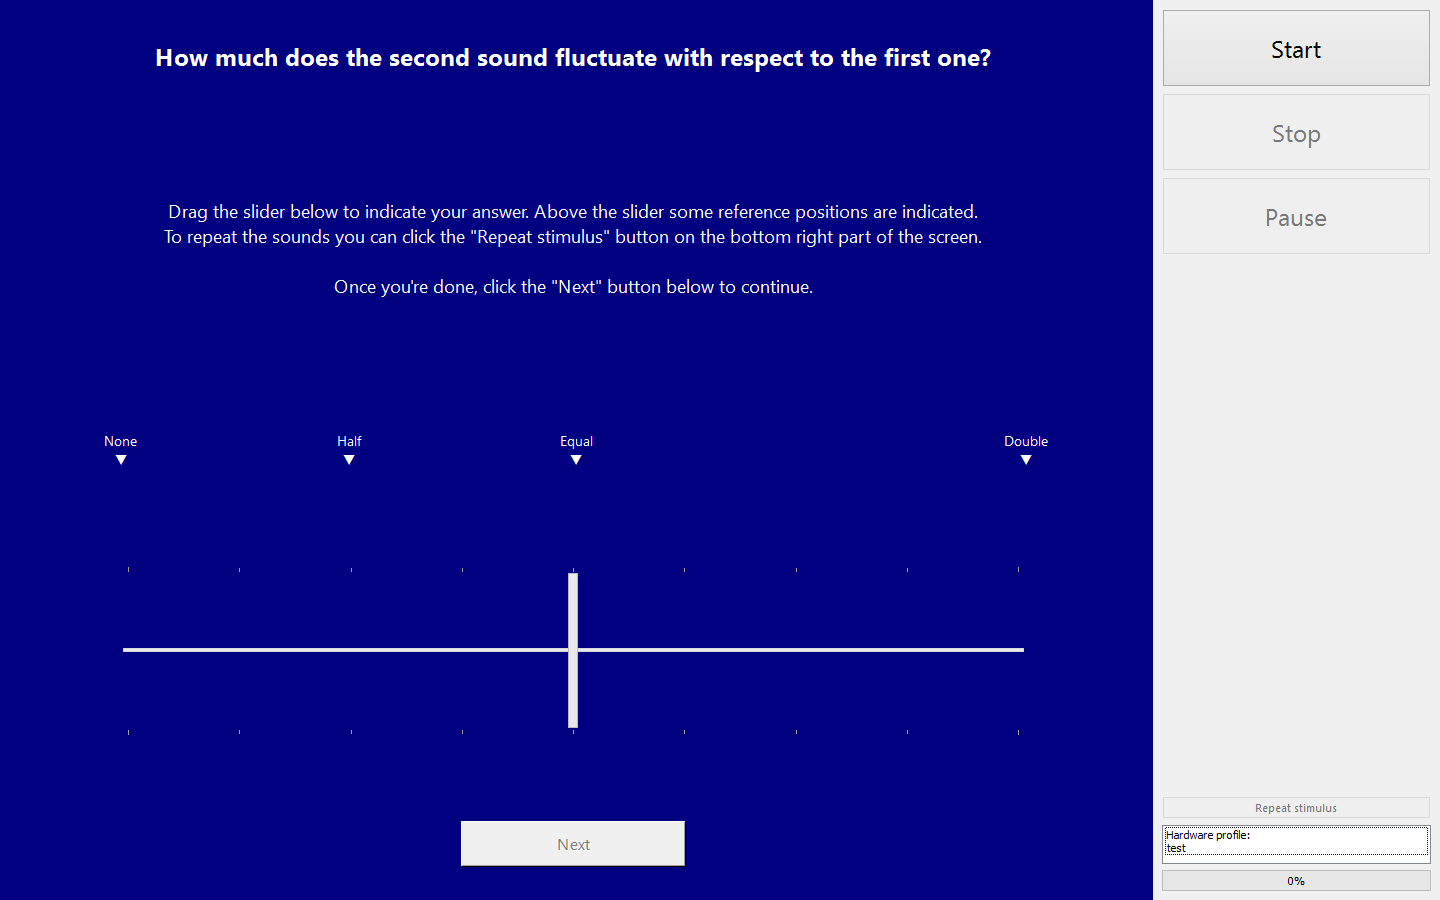
\includegraphics[width=\textwidth]{apex}
  \caption{Screenshot of an experiment section interface}
\label{fig:apex}
\end{figure}

\subsection{Stimuli}
\label{subsec:pilot_stimuli}

All the sounds presented during the experiment consisted of diotic stimuli,
where a monaural stimulus is reproduced for both ears simultaneously. Two
types of stimuli were considered: \gls{AM} tones, \Cref{eq:am}; and \gls{FM}
tones, \Cref{eq:fm}. In these equations, a phase shift of $-\frac{\pi}{2}$ was
introduced to the modulating signal for both tones in order to start the
corresponding modulation at its lowest point. This phase shift is needed to
avoid pops and clicks due to an abrupt onset when presenting the sounds to the
participants. Additionally, a cosine ramp with attack and release times of 25 ms
was applied to the stimuli to further prevent this phenomenon.

\begin{equation}
  x_{am} = A_c \cdot [1 - m_d \cdot \cos(2 \pi f_m t)] \cdot \sin(2 \pi f_c t),
 \text{where } m_d = \frac{A_m}{A_c}
  \label{eq:am}
\end{equation}

\begin{equation}
  x_{fm} = A_c \cdot \sin \{2 \pi [f_c - d_f \cdot \cos(2 \pi f_m t)] t \}
  \label{eq:fm}
\end{equation}

The duration of the stimuli was specified such that it presented at least three
periods of the modulating signal, within a range of values between 2 and
4~seconds. Therefore, stimuli with long periods (e.g., $f_m$ = 0.25~Hz) were
truncated to 4~seconds and stimuli with short periods (e.g., $f_m$ = 32~Hz) were
generated to reach a 2~seconds duration. This was done to maintain a similar
duration among stimuli while keeping the whole experiment duration to an
acceptable value.

Furthermore, the stimuli were generated such that a level of 100 dB SPL value
corresponds to a 0 dBFS value.

\Cref{tab:initial_stimuli} presents all the stimuli used for the different
experimental sections, stating which parameters were fixed and which were varied.

\begin{table}[!ht]
  \centering
  \begin{tabu} to \linewidth{p{2cm}Xp{6cm}}
  \toprule
  \rowfont\bfseries
  \multirow{2}{*}{Section} &
  \multicolumn{2}{c}{Parameters} \\
  \cmidrule{2-3}
  \rowfont\bfseries
  & \multicolumn{1}{c}{Fixed} & \multicolumn{1}{c}{Varied} \\
  \midrule
  AM-fm  & $f_c$ = 1 [kHz]\par SPL = 70 [dB]\par $m_d$ = 40 [dB]
         & $f_m$ = \{0, 0.25, 0.5, 1, 2, 4, 8, 16, 32\} [Hz] \\
  \midrule
  AM-fc  & $f_m$ = 4 [Hz]\par SPL = 70 [dB]\par $m_d$ = 40 [dB]
         & $f_c$ = \{0.125, 0.25, 0.5, 1, 2, 4, 8\} [kHz] \\
  \midrule
  AM-SPL & $f_m$ = 4 [Hz]\par $f_c$ = 1 [kHz]\par $m_d$ = 40 [dB]
         & SPL = \{50, 60, 70, 80, 90\} [dB] \\
  \midrule
  AM-md  & $f_m$ = 4 [Hz]\par $f_c$ = 1 [kHz]\par SPL = 70 [dB]
         & $m_d$ = \{1, 2, 4, 10, 20, 40\} [dB] \\
  \midrule
  FM-fm  & $f_c$ = 1.5 [kHz]\par SPL = 70 [dB]\par $d_f$ = 700 [Hz]
         & $f_m$ = \{0, 0.25, 0.5, 1, 2, 4, 8, 16, 32\} [Hz] \\
  \midrule
  FM-fc  & $f_m$ = 4 [Hz]\par SPL = 70 [dB]\par $d_f$ = 200 [Hz]
         & $f_c$ = \{0.5, 1, 1.5, 2, 3, 4, 6, 8\} [kHz] \\
  \midrule
  FM-SPL & $f_m$ = 4 [Hz]\par $f_c$ = 1.5 [kHz]\par $d_f$ = 700 [Hz]
         & SPL = \{40, 50, 60, 70, 80\} [Hz] \\
  \midrule
  FM-df  & $f_m$ = 4 [Hz]\par $f_c$ = 1.5 [kHz]\par SPL = 70 [dB]
         & $d_f$ = \{16, 32, 100, 300, 700\} [Hz] \\
  \bottomrule
  \end{tabu}
  \caption{Description of initial set of stimuli used per experiment section}
\label{tab:initial_stimuli}
\end{table}

\section{Development}

Not all participants were subjected to the same experimental conditions, and
not all of them used the same version of the experiments.
\Cref{tab:partexpconver} presents the conditions and version to which the
participants were subjected.

\begin{table}[!ht]
  \centering
  \begin{tabu} to \linewidth{XXXX}
    \toprule
    \rowfont\bfseries
    Participant & AM & FM & Version \\
    \midrule
    1 & All & All & 1 \\
    2 & All & None & 1 \\
    3 & All & None & 1 \\
    4 & All & None & 1 \\
    5 & \gls{f_m} & None & 2 \\
    6 & \gls{f_m} & None & 3 \\
    7 & None & \gls{f_m}, \gls{f_c} & 3 \\
    8 & None & All & 3 \\
    9 & None & All & 4 \\
    \bottomrule
  \end{tabu}
  \caption{Participants experimental conditions and versions}
\label{tab:partexpconver}
\end{table}

The experimental procedure was varied during the pilot experiment to accommodate
perceived errors during the realization of them. The first version of the
experiment yielded unsatisfactory results with regards to the relation between
fluctuation strength and modulation frequency (participants 2, 3 and 4). The
procedure was then modified, adding two more AM tones with modulation
frequencies of 64 and 128 Hz. The idea behind the addition of these two tones
was that, if participant have stimuli that are clearly rough, it would be easier
for them to distinguish between a fluctuating and a rough tone. Additionally,
FM tones were included in the training, since up to this point only AM tones
were used in the training phase. This constitutes the second version of the
experiment.

Participant 5 was the only participant that was subjected to version 2 of the
experiment. The results did not show any significant improvements with regard
to the confusion between fluctuation strength and roughness. However, by talking
to the participants it was discovered that the instructions during the training
phase were not clear enough, and this may have affected the results of the
experiment. Several participants associated the rate of change of the stimuli
(modulation frequency in this case) with a bigger fluctuation in the presented
sounds. As so, they tended to deem as highly fluctuating sounds that had a high
modulation frequency. Participants 4 and 5 explicitly stated that they were
counting the number of cycles in the stimuli, due to confusion on what to
answer.

Taking all these comments as feedback, version 3 of the experiment was
elaborated. In this version, explicit instructions regarding the rough tones
were given. It was indicated that the sensation of fluctuation was unrelated to
the apparent `speed' of the stimuli, and that the answers should be intuitive,
based on the arising sensation and not rationalizing any judgment about it
(for instance by counting cycles). Using this approach participants were able to
understand better the fluctuation strength concept, some of them even coming
with analogies to the sensation itself (the sound of an ambulance alarm, the
sound of a washing machine).

The final version, number 4, of the experiment added a small test experiment
before starting the actual experiment sections. This was added as a suggestion
of participant 8, who indicated that although the training phase was effective
in making clear the fluctuation strength concept, it did not show the
participant how to do the expected judgments using the magnitude estimation
procedure. Moreover, a latin square randomization approach was used, rotating
the order of the experimental sections for each participant. The purpose of this
was to distribute possible learning effects of participants among the
experimental conditions.

\section{Results}

The following are the results of all the participants grouped together by
experiment. In the appendix the individual results can be found. In
\Cref{fig:pilot_AM_all_comparison,fig:pilot_FM_all_comparison} the error bars
indicate the interquartile range and the marker indicates the median value.

\begin{pilotresults}

\myfigurequad%
  {AM-fm_all_standards}
  {AM-fc_all_standards}
  {AM-SPL_all_standards}
  {AM-md_all_standards}
  {
    \caption{Pilot results --- Relative fluctuation strength for AM tones}
\label{fig:pilot_AM_all_comparison}
  }

\myfigurequad%
  {FM-fm_all_standards}
  {FM-fc_all_standards}
  {FM-SPL_all_standards}
  {FM-df_all_standards}
  {
    \caption{Pilot results --- Relative fluctuation strength for FM tones}
\label{fig:pilot_FM_all_comparison}
  }

\end{pilotresults}

\section{Conclusions}

From the obtained data it can be concluded that the main problem when dealing
with the perceptual attribute of fluctuation strength is its ambiguity and
confusion with the perceptual attribute of roughness perceptual. The proposed
training phase was effective in clarifying the concept to participants, by
adding stimuli with a clear rough sensation, and by clearly instructing them on
what the sensation is about. It should be noted that only with regard to
modulation frequency this confusion arises, the other parameters do not present
this particularity and as so it was not necessary to adapt the experimental
procedure with them.

\end{document}
